\section{Porównanie twarzy}
Twarze rozpoznane na zdjęciu zostają przekazane w celu ich porównania z twarzami dostępnymi w bazie. Porównywanie twarzy opiera się o szereg algorytmów.

\subsection{Kowariancja}
Kowariancja jest miarą tego, jak dalece wartości dwóch zmiennych losowych zmieniają się razem. Jeśli zmienne zachowują się podobnie, to kowariancja jest liczbą dodatnia, w przeciwnym razie kowariancja jest ujemna.
Macierz kowariancji to macierz której elementem na miejscu (i,j) jest kowariancja pomiędzy i-tym oraz j-tym elementem wektora losowego.   

\subsection{Analiza głównych składowych (PCA)}
Statystyczna metoda służąca odnajdywaniu struktur w zbiorze zmiennych losowych. Celem PCA jest przekształcenie zbioru obserwacji prawdopodobnie skorelowanych ze sobą zmiennych w zbiór wartości nieskorelowanych zmiennych zwanych głównymi składowymi. Transformacja ta jest zdefiniowana w taki sposób, że pierwsza główna składowa ma jak największą wariancję (czyli wyjaśnia tak  dużą część  zmienności danych jak to tylko możliwe), a każdy kolejny element ma jak największą wariancję pod warunkiem, że jest nie jest skorelowany z poprzednią składową.

\subsection{Eigenface}
Eigenface, lub twarze własne, to zbiór wektorów własnych używany przy komputerowym rozpoznaniu twarzy. Zbiór twarzy własnych może zostać wygenerowany przez wykonanie procedury PCA na dużym zbiorze obrazów ludzkich twarzy. Twarze własne można traktować jak zbiór "standaryzowanych składników twarzy". Każda ludzka twarz może być pojmowana jako kombinacja tych standardowych twarzy. Przykładowo czyjaś twarz może być kompozycją twarzy uśrednionej plus 10\% cech z twarzy własnej 1, 1,55\% z twarzy własnej nr 2 oraz nawet 3\% z twarzy własnej 3. 

\begin{figure}[h]
\centering
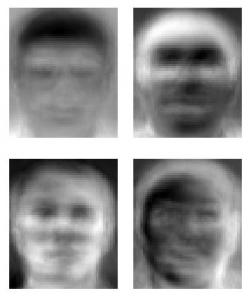
\includegraphics[scale=0.5]{./eigenface.jpg}
\caption[Twarze własne, przykłady]{Przykłady twarzy własnych z laboratorium AT\&T w Cambridge}
\end{figure}

Dzięki przechowywaniu twarzy nie jako pliku graficznego, a jako listy pewnych wartości, rozmiar pliku jest niewielki. Stworzone twarze własne będą ukazywać się jako jasne  ciemne obszary układające się w pewien określony zbiór.

\subsection{Algorytm k najbliższych sąsiadów}
Jest to algorytm uzywany w statystyce do prognozowania wartości pewnej zmiennej losowej, jednak może być również używany do klasyfikacji. Aby polepszyć działanie algorytmu kNN powszechnie stosowaną techniką jest \textbf{standaryzacja} lub \textbf{normalizacja} danych. Standaryzacja polega na doprowadzeniu do sytuacji w której wartość średnia poszczególnej cechy ma wartość 0 a odchylenie standardowe = 1. Normalizacja to  doprowadzenie do sytuacji w której wartości zmiennej należą do przedziału [0,1]
\newline \\
\textbf{Uczenie}:
\begin{enumerate}
  \item Dokonaj alternatywnie: standaryzacji/normalizacji/pozostaw dane jakie są
  \item Zapamiętaj cały zbiór treningowy
\end{enumerate}
\textbf{Testowanie}:
\begin{enumerate}
  \item Dokonaj standaryzacji/normalizacji/pozostaw dane jakie są (testowanie)
  \item Policz odległości pomiędzy wektorem testowym a wszystkimi wektorami zbioru treningowego
  \item Posortuj odległości od największej do najmniejszej
  \item Zobacz etykiety  k – najbliższych wektorów do wektora testowego.  Zrób histogram częstości poszczególnych etykiet spośród „k-najbliższych” (Policz ile i których etykiet było spośród k najbliższych)
  \item Przypisz najczęściej występującą etykietę jako etykietę wektora testowego 
  \item Jeśli wystąpił impas (dwie klasy miały taką samą liczbę głosów) rozwiąż problem losowo
\end{enumerate}
\pagebreak[4]
